%&"ml"
\begin{document}
    \title{复习}
    \maketitle
    \section{聚类}
    \subsection{k-means}
   	\begin{algorithm}[h]
   		\caption{k-means}
   		初始化均值点 $\mu_1,\cdots,\mu_k$\;
   		\Repeat{$\mu_i$分配不变}{
   			\ForEach{$x_n\in X$}{
   				\ForEach{$k$}{
	   				\begin{equation}
	   					\begin{aligned}
	   						r_{nk} = \begin{cases}
	   							1, &\text{if } k=\arg\min_j\lVert x_n - \mu_j\rVert^2\\
	   							0, &\text{otherwise.}
	   						\end{cases}
	   					\end{aligned}
	   				\end{equation}
	   			}
   			}
   			\ForEach{$\mu_n$}{
   				\begin{equation}
   					\mu_i\leftarrow \frac{\sum_n r_{nk}x_n}{\sum_n b_{nk}}
   				\end{equation}	
   			}
   		}
 	\end{algorithm}
	\subsection{GMM}
	\begin{algorithm}[ht]
		\caption{GMM}
	 初始化均值矩阵 $\bm{\mu}_k$,协方差矩阵 $\bm{\Sigma}_k$,混合参数 $\pi_k$,初始化对数似然值\;
	\Repeat{$\ln p(\bm{X}|\bm{\mu},\bm{\Sigma},\bm{\pi})=\sum_{n=1}^N\ln\left\{\sum_{k=1}^K\pi_k\mathcal{N}(\bm{x}_n|\bm{\mu}_k,\bm{\Sigma}_k)\right\}$没有明显变化}{
		\For{$n\leftarrow 1$ to $N$}{
			\For{$k\leftarrow 1$ to $K$}{
				\begin{equation}
					\gamma_{nk}^{(t)}\leftarrow \frac{\pi_k\mathcal{N}(\bm{x}_n|\bm{\mu}_k,\bm{\Sigma}_k)}{\sum_{j=1}^K\pi_j\mathcal{N}(\bm{x}_n|\bm{\mu}_j,\bm{\Sigma}_j)}
				\end{equation}
			}
		}
		\For{$k\leftarrow 1$ to $K$}{
			\begin{align}
				N_k&=\sum_{n=1}^N\gamma_{nk}\\
				\bm{\mu}_k^{(t+1)}&\leftarrow\frac{1}{N_k}\sum_{n=1}^N\gamma_{nk}^{(t)}\bm{x}_n\\
				\bm{\Sigma}_k^{(t+1)}&\leftarrow\frac{1}{N_k}\sum_{n=1}^N\gamma_{nk}^{(t)}(\bm{x}_n-\bm{\mu}_k^{(t+1)})(\bm{x}_n-\bm{\mu}_k^{(t+1)})^T\\
				\pi_k&\leftarrow\frac{N_k}{N}
			\end{align}
		}
	}
	\Return{$\bm{\mu},\bm{\Sigma}$}
	\end{algorithm}

	\subsection{GDA}
	
	Bernoulli
%	\begin{align*}
%		p(y=1|\phi) &= \phi\\
%		p(y=0|\phi) &= 1-\phi\\
%		p(y|\phi) &= \phi^y(1-\phi)^{1-y}\\
%		&=\exp\left(y\log\phi+(1-y)\log(1-\phi)\right)\\
%		&=\exp\left(y\left(\log\frac{\phi}{1-\phi}\right)+\log(1-\phi)\right)
%	\end{align*}

	\begin{align*}
		y&\sim \text{Bernoulli}(\phi)\\
		x|y=0&\sim\mathcal{N}(\mu_0,\Sigma)\\
		x|y=1&\sim\mathcal{N}(\mu_1,\Sigma)
	\end{align*}

	\begin{align*}
		p(y)&=\phi^y(1-\phi)^{1-y}\\
		p(x|y=0)&=\frac{1}{(2\pi)^{d/2}|\Sigma|^{1/2}}\exp\left(-\frac{1}{2}(x-\mu_0)^\top\Sigma^{-1}(x-\mu_0)\right)\\
		p(x|y=1)&=\frac{1}{(2\pi)^{d/2}|\Sigma|^{1/2}}\exp\left(-\frac{1}{2}(x-\mu_1)^\top\Sigma^{-1}(x-\mu_1)\right)
	\end{align*}

	\begin{equation}
		\log\int p(x|y)p(y)dy
	\end{equation}

	\begin{align*}
		\phi&=\frac{1}{n}\sum_{i=1}^n |y_i=1|\\
		\mu_0&=\frac{\sum_{i=1}^n|y_i=0|x_i}{\sum_{i=1}^n|y_i=0|}\\
		\mu_1&=\frac{\sum_{i=1}^n|y_i=1|x_i}{\sum_{i=1}^n|y_i=1|}\\
		\Sigma&=\frac{1}{n}\sum_{i=1}^n(x_i-\mu_{y_i})(x_i-\mu_{y_i})^\top
	\end{align*}

	\subsection{EM}
	\begin{align}
		p(x,z)&=p(x|z)p(z)\\
		p(x)&=\sum_z p(x,z)=\sum_z p(x|z)p(z)
	\end{align}
	
	\begin{algorithm}[h]
		\caption{EM}
		初始化参数 $\theta^\text{old}$\;
		E 步:评估 $p(Z|X,\theta^\text{old})$\;
		M 步:得到新的参数
		\begin{align*}
			\theta^\text{new}&={\arg\max}_\theta Q(\theta,\theta^\text{old})\\
			Q(\theta,\theta^\text{old})&=\sum_{Z}p(Z|X,\theta^\text{old})\ln p(X,Z|\theta)
		\end{align*}
		查看对数似然值是否收敛,不收敛返回步骤 2。
	\end{algorithm}

%	\begin{tikzpicture}
%		\node (v1) at (0.5,1.5) {$z$};
%		\node (v2) at (0.5,-0.5) {$x$};
%		\draw[bend left,-latex]  (v1) edge node[right] {$p(x|z)$} (v2);
%		\draw[bend left,-latex]  (v2) edge node[left] {$p(z|x)$} (v1);
%		\node [right of=v1] {$p(z)$};
%	\end{tikzpicture}

	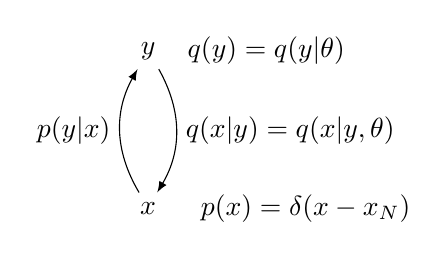
\begin{tikzpicture}
		\node (v1) at (0.5,1.5) {$y$};
		\node (v2) at (0.5,-0.5) {$x$};
		\draw[bend left,-latex]  (v1) edge node[right] {$q(x|y)=q(x|y,\theta)$} (v2);
		\draw[bend left,-latex]  (v2) edge node[left] {$p(y|x)$} (v1);
		\node [right of=v1,xshift=0.5cm] {$q(y)=q(y|\theta)$};
		\node [right of=v2,xshift=1cm] {$p(x)=\delta(x-x_N)$};
	\end{tikzpicture}

\clearpage

	\paragraph{Jenson's Inequation Method}
	
	\begin{align*}
		\log(P(x|\theta)) &= \log\left(\sum_y P(x,y|\theta)\right) \\
		&=\log\left(\sum_y q(y) \frac{P(x,y|\theta)}{q(y)}\right)\\ 
		&\geq E_q\left[\log\frac{P(x,y|\theta)}{q(y)} \right]\\
		&\geq E_q\left[\log\frac{P(y|x,\theta)P(x|\theta)}{q(y)}\right]\\
		&\geq E_q[\log(P(x|\theta))] - E_q\left[\log\frac{q(y)}{P(y|x,\theta))})\right]\\
		&\geq E_q[\log(P(x|\theta))] - KL(q(y)\Vert P(y|x,\theta))\\
		&\geq \fbox{$\log(P(x|\theta)) - KL(q(y)\Vert P(y|x,\theta))$}
	\end{align*}

	\begin{align*}
		\log(P(x|\theta))&\geq E_q\left[\log\frac{P(x,y|\theta)}{q(y)}\right]\\
		&\geq E_q\left[\log(P(x,y|\theta))\right] - E_q[\log(q(y))]\\
		&\geq E_q\left[\log(P(x,y|\theta))\right] + H(q(y))
	\end{align*}

	\paragraph{KL Matching}
	
	\begin{equation}
		p(x)=\delta(x-\mathbf{x}_N)
	\end{equation}
	
	\begin{align*}
		\max_\theta q(x|\theta) &=\max_\theta  \int q(x|y)q(y)dy
	\end{align*}
	
	\begin{equation}
		p(x)\leftrightarrow q(x|\theta)
	\end{equation}
	
	\begin{align*}
		\min_{\theta}KL(p||q)&=\min_{\theta}\int p(x)\log \frac{p(x)}{q(x|\theta)}
		\\&=\min_{\theta}\int p(x)\log p(x) - \int p(x)\log q(x|\theta)
		\\&=\min_{\theta}\int \frac{1}{N}\sum_{t=1}^N \delta(x-x_t)\log q(x|\theta)
		\\&=\frac{1}{N}\sum_{t=1}^N\log q(x_t|\theta) && \int \delta(x)f(x) = f(0)
	\end{align*}

	\begin{equation}
		p(x)p(y|x)\leftrightarrow q(x|y,\theta)q(y|\theta)
	\end{equation}
	
	\begin{align*}
		\max F(p(y|x),\theta)&=\int p(x)p(y|x)\log\frac{q(x|y,\theta)q(y|\theta)}{p(y|x)}\\
		&=\int p(x)p(y|x)\log\frac{q(x|y,\theta)q(y|\theta)}{q(x|\theta)}\frac{q(x|\theta)}{p(y|x)}\\
		&=\int p(x)p(y|x)\left[\log q(x|\theta)-\log\frac{p(y|x)}{q(y|x,\theta)} \right]\\
		&=\frac{1}{N}\sum_{t=1}^N\log q(x_t|\theta) - \int p(x)\cdot KL(p(y|x)||q(y|x,\theta))\\
		&\leq\log q(x|\theta) @ [p(y|x)=q(y|x,\theta)]
	\end{align*}


fix $p(y|x)$, $F=\int p(y|x)\log[q(x|y,\theta)q(y|\theta)]$

E Step -- fix $\theta: p(y|x)=q(y|x,\theta)$

M Step -- fix $p(y|x)$, 
$$F=\int p(y|x)\log [q(x|y,\theta)q(y|\theta)]) - \int p(y|x)^\text{old}\log p(y|x)$$

$\max_\theta F(P(y|x)^\text{old},\theta)$

\section{贝叶斯学习}

Bayes rule:
\begin{equation}
	P(\Theta|X)=\frac{P(X|\Theta)P(\Theta)}{P(X)}
\end{equation}

Bayes learning - Maximum A Posteriori (MAP)

引入先验知识。

\begin{equation}
	\max_{\Theta} \log p(\Theta|X) = \max_{\Theta} (\log p(X|\Theta) + \log p(\Theta) )
\end{equation}

例子:

\begin{align*}
	p(x|\Theta) &= G(x|\mu,\Sigma) \\
	p(\mu) & = G(\mu|\mu_0,\sigma_0^2)\\
	p(\mu|x)&\propto p(x|\mu,\Sigma)p(\mu)\\
	&=\prod_{t=1}^{N}p(x_t|\mu,\Sigma)p(\mu)&&\text{(i.i.d.)}\\
	\log p(\mu|x)\propto &\sum_{t=1}^{N}\log G(x_t|\mu,\Sigma) + \log G(\mu|\mu_0, \sigma_0^2 I)\\
	=&\sum_{t=1}^{N}\left\{ -\frac{d}{2}\log (2\pi) -\frac{1}{2}\log |\Sigma| -\frac{1}{2}(x_t-\mu)^\top\Sigma^{-1}(x_t-\mu) \right\}\\
	&-\frac{d}{2}\log(2\pi)-\frac{1}{2}\log|\sigma_0^2I|-\frac{1}{2}(\mu-\mu_0)^\top\sigma_0^{-2}I(\mu-\mu_0)
\end{align*}

\begin{align*}
	\frac{\partial \log p(\mu|x)}{\partial \mu} &= \sum_{t=1}^N\left\{\frac{1}{2}\times 2\Sigma^{-1}(x_t-\mu)(-1)\right\} - \frac{1}{2}\times 2\sigma_0^{-2}(\mu-\mu_0)\\
	&=\Sigma^{-1}(N\bar{x}-N\mu)-\sigma_0^{-2}\mu + \sigma_0^{-2}\mu_0=0\\
	\mu&=(N\Sigma^{-1}+\sigma_0^{-2}I)^{-1}(N\Sigma^{-1}\bar{x}+\sigma_0^{-2}\mu_0)\\
	&=(\sigma_0^2\Sigma^{-1}+\frac{1}{N}I)^{-1}(\sigma_0^2\Sigma^{-1}\bar{x}+\frac{1}{N}\mu_0)
\end{align*}

For a fixed $\sigma_0^2$, $N\rightarrow 0$, $\mu\rightarrow(\sigma_0^2\Sigma^{-1})^{-1}(\sigma_0^2\Sigma^{-1})\bar{x}=\bar{x}$

For a fixed $N\ll +\infty, \sigma_0^2\rightarrow 0$,$\mu\rightarrow (\frac{1}{N}I)^{-1}(\frac{1}{N}\mu_0)=\mu_0$

\begin{equation}
	-2\log p(\mu|X) \propto \sum_t \lVert x_t-\mu \rVert^2+\lVert\mu-\mu_0\rVert^2
\end{equation}

$\max_k q(x|k)=\int q(x|\theta)q(\theta)d\theta$ marginal likelihood

ML $\log q(x|\theta)$

BL $\log q(x|\theta)q(\theta)=\log q(x|\theta) + \log q(\theta)$ 后项为正则化项

\subsection{VAE}

\begin{align}
	\log P(X) - \mathcal{D}[Q(z|x)\Vert P(z|X)] &= E_{z\sim Q}[\log P(X|z)] - \mathcal{D}[Q(z|X)\Vert P(z)]
\end{align}

\begin{align*}
	\log P(x) &= \int_z q(z|x)\log P(x)dz\\
	&=\int_z q(z|x)\log\frac{P(z,x)}{P(z|x)}dz\\
	&=\int_z q(z|x)\log\left(\frac{P(z,x)}{q(z|x)}\frac{q(z|x)}{P(z|x)}\right)dz\\
	&=\int_z q(z|x)\log\frac{P(z,x)}{q(z|x)}dz + \int_z q(z|x)\log\frac{q(z|x)}{P(z|x)}dz\\
	&=\int_z q(z|x)\log\frac{P(z,x)}{q(z|x)}dz + KL(q(z|x)\Vert P(z|x))\\
	&=\int_z q(z|x)\log\frac{P(x|z)P(z)}{q(z|x)}dz + KL(q(z|x)\Vert P(z|x))\\
	&=\int_z q(z|x)\log P(x|z)dz - \int_z q(z|x)\log\frac{q(z|x)}{P(x|z)}dz + KL(q(z|x)\Vert P(z|x))\\
	&=\int_z q(z|x)\log P(x|z)dz - KL(q(z|x)\Vert P(x|z)) + KL(q(z|x)\Vert P(z|x))
\end{align*}

\paragraph{Reparameterization}

\begin{align}
	z&\sim \mathcal{N}(z|\mu,\sigma^2)\\
	z&=\mu+\sigma\cdot\epsilon\\
	\epsilon&\sim\mathcal{N}(\epsilon|0,1)
\end{align}

虽然VAE比普通的AE模型训练出来的效果要好很多,但是训练过VAE模型的人都知道,它生成出来的图片相对GANs那种直接利用对抗学习的方式会比较模糊,这是由于它是通过直接计算生成图片和原始图片之间的均方误差,所以得到的是一张“平均图像”。

Conditional VAE given $y_i$

\subsection{GAN}

\begin{equation}
	\min_G\max_D V(D,G) = E_{x\sim p_\text{data}(x)}[\log D(x)] + E_{z\sim p_z(z)}[\log(1-D(G(z)))]
\end{equation}

\begin{align*}
	C(G) &= E_{x\sim p_\text{data}}\left[\log\frac{p_\text{data}(x)}{p_\text{data}(x)+p_g(x)}\right]+E_{x\sim p_g}\left[\log\frac{p_g(x)}{p_\text{data}(x)+p_g(x)}\right] \\
	&=-\log(4)+KL\left(p_\text{data}\left\Vert\frac{p_\text{data}+p_g}{2}\right.\right)+KL\left(p_g\left\Vert\frac{p_\text{data}+p_g}{2}\right.\right)\\
	&=-\log(4)+2\cdot JSD(p_\text{data}\Vert p_g)
\end{align*}


\section{数据降维}

\subsection{PCA}

    \begin{algorithm}
	\caption{特征值分解 PCA}
	\KwIn{数据集 $\mathbf{X}=\{\mathbf{x}_1,\mathbf{x}_2,\cdots,\mathbf{x}_N\}, \mathbf{x}_t\in\mathbb{R}^{n\times 1}$}
	\KwOut{主成分 $\mathbf{w}$}
	\BlankLine
	计算平均值 $\mathbf{\mu}\leftarrow\frac{1}{N}\sum_{i=1}^N \mathbf{x}_i$\;
	\ForEach{$i\leftarrow 1$ to $N$}{
		$\mathbf{x}_i\leftarrow \mathbf{x}_i - \mathbf{\mu}$\;
	}
	计算散度矩阵 $C\leftarrow XX^T$\;
	特征值分解求 $C$ 的特征值 $\lambda_1\geq\lambda_2\geq\cdots\geq\lambda_n$ 与对应的特征向量 $\mathbf{v}_1,\mathbf{v}_2,\cdots,\mathbf{v}_n$\;
	选取最大的特征值对应的特征向量与数据的乘积即为主成分 $\mathbf{w}\leftarrow\mathbf{v_1}^T\mathbf{X}$\;
	\Return{$\mathbf{w}$}\;
\end{algorithm}

    \begin{algorithm}
	\caption{奇异值分解}
	\KwIn{数据集 $\mathbf{X}=\{\mathbf{x}_1,\mathbf{x}_2,\cdots,\mathbf{x}_N\}, \mathbf{x}_t\in\mathbb{R}^{n\times 1}$}
	\KwOut{主成分 $\mathbf{w}$}
	\BlankLine
	计算平均值 $\mathbf{\mu}\leftarrow\frac{1}{N}\sum_{i=1}^N \mathbf{x}_i$\;
	\ForEach{$i\leftarrow 1$ to $N$}{
		$\mathbf{x}_i\leftarrow \mathbf{x}_i - \mathbf{\mu}$\;
	}
	奇异值分解 $\mathbf{X}=\mathbf{U}\mathbf{\Sigma}\mathbf{V}^T$\;
	两边同乘 $\mathbf{U}^T$,$\mathbf{U}^T\mathbf{X}=\mathbf{\Sigma}\mathbf{V}^T$ 得到压缩数据\;
	选取 $\mathbf{\Sigma}\mathbf{V}^T$ 中最大的那一个奇异值(习惯上应为左上角的值)对应的向量(一般为第一行)即为主成分 $\mathbf{w}$\;
	\Return{$\mathbf{w}$}\;
\end{algorithm}

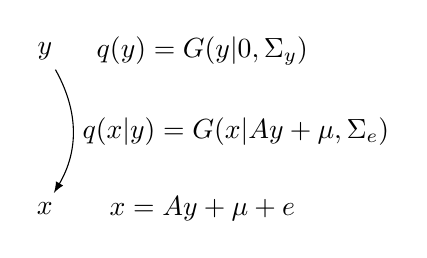
\begin{tikzpicture}
	\node (v1) at (0.5,1.5) {$y$};
	\node (v2) at (0.5,-0.5) {$x$};
	\draw[bend left,-latex]  (v1) edge node[right] {$q(x|y)=G(x|Ay+\mu,\Sigma_e)$} (v2);
%	\draw[bend left,-latex]  (v2) edge node[left] {$p(y|x)$} (v1);
	\node [right of=v1,xshift=1cm] {$q(y)=G(y|0,\Sigma_y)$};
	\node [right of=v2,xshift=1cm] {$x=Ay+\mu+e$};
\end{tikzpicture}

\begin{align*}
	\int q(x,y)dy &= q(x|\theta) = G(x|\mu_x,\Sigma_x)\\
	\mu_x &= E[x] = AE[y] + \mu + E[e] = \mu  && \Sigma_y = I\\
	\Sigma_x &= \text{cov}(x) \\
	&=E[(x-\mu)(x-\mu)^\top]\\
	&=E[(Ay+e)(Ay+e)^\top]\\
	&=E[Ayy^\top A+Aye^\top + e(Ay)^\top+ee^\top ]\\
	&= E[Ayy^\top A+ee^\top]\\
	&=A\Sigma_y A^\top + \Sigma_e
\end{align*}

%A^TR^TRA

\begin{equation}
	\frac{\sum_{i=1}^{d^\prime}\lambda_i}{\sum_{i=1}^d\lambda_i}\geq t
\end{equation}


\subsection{FA}

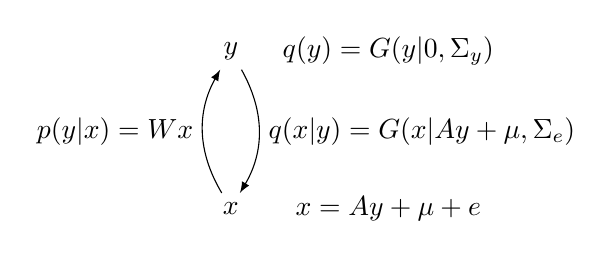
\begin{tikzpicture}
	\node (v1) at (0.5,1.5) {$y$};
	\node (v2) at (0.5,-0.5) {$x$};
	\draw[bend left,-latex]  (v1) edge node[right] {$q(x|y)=G(x|Ay+\mu,\Sigma_e)$} (v2);
	\draw[bend left,-latex]  (v2) edge node[left] {$p(y|x)=Wx$} (v1);
	\node [right of=v1,xshift=1cm] {$q(y)=G(y|0,\Sigma_y)$};
	\node [right of=v2,xshift=1cm] {$x=Ay+\mu+e$};
\end{tikzpicture}

E-Step: 
\begin{align*}
	q(x,y) &= \frac{1}{()}e^{-\frac{1}{2}(x-Ay-\mu)^\top\Sigma_x^{-1}(x-Ay-\mu)}\frac{1}{()}e^{-\frac{1}{2}y^\top I^{-1}y}\\
	&\propto \exp\left\{-\frac{1}{2}\left[y^\top A^\top \Sigma_e^{-1} Ay - 2y^\top A^\top \Sigma_e^{-1}(x-\mu) + (x-\mu)^\top\Sigma_e^{-1}(x-\mu)\right]-\frac{1}{2}y^\top I^{-1}y
	\right\}\\
	&=\exp\left\{\frac{1}{2}\left[y^\top(A^\top\Sigma_e^{-1}A+I^{-1})y-2y^\top A^\top \Sigma_e^{-1}(x-\mu)\right] + \cdots\right\}
\end{align*}

\begin{align*}
p(y|x)=q(y|x,\theta)&=\frac{q(x|y)q(y)}{q(x|\theta)}\\
&=\frac{q(x,y)}{q(x|\theta)}\\
&=G(y|\mu_{y|x},\Sigma_{y|x})\\
&\propto \exp\left\{-\frac{1}{2}(y-\mu_{y|x})^\top\Sigma_{y|x}^{-1}(y-\mu_{y|x})\right\}\\
&=\exp\left\{-\frac{1}{2}y^\top\Sigma_{y|x}^{-1}y-2y^T\Sigma_{y|x}^{-1}\mu_{y|x}+\mu_{y|x}^{-1}\mu_{y|x} \right\}\\
\end{align*}

\begin{align*}
	&\Rightarrow \begin{cases}
		\Sigma_{y|x}^{-1} = A^\top\Sigma_e^{-1}A + I^{-1}\\
		\Sigma_{y|x}^{-1}\mu_{y|x}=A^\top\Sigma_e^{-1}(x-\mu)
	\end{cases} \text{归一化 $x$ 则 $y$ 系数一致}\\
	&\Rightarrow \begin{cases}
		\Sigma_{y|x} = (A^\top\Sigma_e^{-1}A + I)^{-1}\\
		\mu_{y|x} = (A^\top \Sigma_e^{-1} A +I)^{-1}A^\top \Sigma_e^{-1}(x-\mu) = (A^\top A+\sigma_e^2 I)^{-1}A^\top (x-\mu)
	\end{cases}\\
	&\Rightarrow W = (A^\top A+\sigma_e^2 I)^{-1}A^\top \approx A^{-1}\text{伪逆}
\end{align*}

M-Step:
$\max_\Theta Q(p^\text{old}(y|x),\Theta])$

\begin{align*}
	Q &= \int p^\text{old}(y|x)\cdot\ln[G(y|0,I)G(x|Ay+\mu,\sigma^2 I)]dy\\
	A_\text{new}&=\left(\sum_{t=1}^N x_t(E[y|x_t])^\top\right)\left(\sum_{t=1}^N E[yy^\top|x_t]\right)^{-1}\\
	\sigma^2_\text{new}&=\frac{1}{Nd}\text{Tr}\left\{\sum_{t=1}^N(x_tx_t^\top-A_\text{new}E[y|x_t]x_t^\top)\right\}
\end{align*}

\begin{align*}
	q(x|\theta) &= G(x|\mu,\Sigma_x) = G(x|AA^\top + \sigma^2 I)\\
	\text{i.i.d.} \{x_t\}_{t=1}^N, \max_\theta\prod_{t=1}^N q(x_t|\theta)&\Leftrightarrow\max_\theta\sum_{t=1}^N \log q(x_t|\theta)\\
	&\Rightarrow \begin{cases}
		\mu = \frac{1}{N}\sum_{t=1}^N x_t\\
		\Sigma_x =UDU^\top = \frac{1}{N}\sum_t (x_t-\mu)(x_t-\mu)^\top =AA^\top +\sigma^2 I
	\end{cases}
\end{align*}

\paragraph{Bias-variance decompostion}

\begin{align*}
	x &= f(y)+\epsilon \\
	E\left[\left(x-\hat{f}(y)\right)^2\right]&=E[x^2+\hat{f}^2-2x\hat{f}]\\
	&=\text{Var}[\epsilon]+\text{Var}[\hat{f}]+\text{Bias}^2[\hat{f}]
\end{align*}

\paragraph{Model Selection}

\begin{align*}
	J_\text{AIC}&=\ln p(X_N|\hat{\Theta}_k)-d_k\\
	J_\text{BIC}&=\ln p(X_N|\hat{\Theta}_k)-\frac{1}{2}d_k\ln N
\end{align*}

\subsection{VFA (Variational FA)}

$p(x)p(y|x,\theta)p(\theta|x)\leftrightarrow q(x|y,\theta)q(y|\theta)q(\theta)$

$$
\begin{aligned}
	F&=\int p(x)p(y|x,\theta)p(\theta|x)\log\frac{q(x|y,\theta)q(y|\theta)q(\theta)}{p(y|x,\theta)p(\theta|x)}\\
	&=\int p(x)p(y|x,\theta)p(\theta|x)\log\frac{q(x|y,\theta)q(y|\theta)}{q(x|\theta)}\frac{q(x|\theta)q(\theta)}{p(y|x,\theta)p(\theta|x)}\\
	&=\int p(x)p(y|x,\theta)p(\theta|x)\log\frac{q(y|x,\theta)}{p(y|x,\theta)}\frac{q(x|\theta)q(\theta)}{q(x|k)p(\theta|x)}q(x|k)\\
	&=\int p(x)p(y|x,\theta)p(\theta|x)\left(\log\frac{q(y|x,\theta)}{p(y|x,\theta)}+\log\frac{q(\theta|x)}{p(\theta|x)}+\log q(x|k)\right) & \text{VBEM}\\
\end{aligned}
$$

\subsection{ICA}

\begin{equation}
	x=As
\end{equation}

\begin{algorithm}[h]
	\caption{FastICA}
	Choose an initial weight vector $\mathbf{w}$\;
	Let $\mathbf{w}^+=E\{\mathbf{w}g(\mathbf{w^\top x})\} - E\{g^\prime (\mathbf{w^\top x})\}\mathbf{w}$\;
	Let $\mathbf{w}=\frac{\mathbf{w}^+}{\lVert\mathbf{w}^+\rVert}$\;
	If not converged, go back to 2.
\end{algorithm}

\section{SVM}


基础的支持向量机(Support Vector Machine, SVM)是一种二分类模型,是一种定义在特征空间上的间隔最大的分类器模型。
对于本文的三分类问题,将会采用一对一策略(one-vs-one scheme),分解为三个二分类问题,组合这些分类器进行求解。

本文使用核函数方法映射到另一个特征空间进行分类,采用软间隔方法允许一定的误差、配合 $L_2$ 正则化降低过拟合风险\cite{sklearn}:
\begin{equation}\label{eq:svc}
	\begin{aligned}
		\min_{\textbf{w},b,\xi}\quad&\frac{1}{2}\left\Vert\textbf{w}\right\Vert^2 + C\sum_{i=1}^n \xi_i\\
		\text{subject to }& y_i(\mathbf{w}^\top\mathbf{x}_i+b)\geq 1-\xi_i\\
		&\xi_i\geq 0,\quad i=1,2,\cdots,m
	\end{aligned}
\end{equation}
其中 $C$ 为正则化系数,$\xi_i$ 为“松弛变量”(slack variables),\eqref{eq:svc} 的对偶问题为
\begin{equation}
	\begin{aligned}
		\min_{\alpha}\quad&\frac{1}{2}\alpha^\top \mathbf{Q}\alpha - \mathbf{e}^\top\alpha\\
		\text{subject to }& y^\top\alpha = 0 \\
		&0\leq \alpha_i\leq C,\quad i=1,\cdots,n
	\end{aligned}
\end{equation}
其中
\begin{equation}
	\mathbf{Q} = \left(Q_{ij}\right)_{n\times n} = \left(y_iy_j\kappa(\mathbf{x}_i,\mathbf{x}_j)\right)_{n\times n}
\end{equation}
这里 $\kappa(\mathbf{x}_i,\mathbf{x}_j)=\phi(\mathbf{x}_i)^\top\phi(\mathbf{x}_j)$ 为核函数。
%
%而 SVM 又可以分为线性 SVM 和非线性 SVM。因此在基线测试方面,本文将对 \verb"linear" 核与 \verb"sigmoid" 核的结果进行对比,采用的核函数如表 \ref{tab:kernel} 所示\cite{ml}。而为了提升分类效果,本文采用的 SVM 方法还会对数据输入进行归一化和 PCA 降维处理。
%
%\begin{table}[h]
%	\centering
%	\caption{核函数}
%	\label{tab:kernel}
%	\begin{tabular}{cc}
%		\toprule
%		类型 & 核函数 \\
%		\midrule
%		\verb"linear" & $\kappa(\mathbf{x}_i,\mathbf{x}_j)=\mathbf{x}_i^\top\mathbf{x}_j$\\
%		\verb"sigmoid" & $\kappa(\mathbf{x}_i,\mathbf{x}_j)=\tanh\left(\beta\mathbf{x}_i^\top\mathbf{x}_j+\theta\right)$\\
%		\bottomrule
%	\end{tabular}
%\end{table}



\begin{table}
	\caption{仅分类}
	\begin{tabular}{l*{2}{l}}
		\toprule
		 & \multicolumn{1}{c}{k-means}  & \multicolumn{1}{c}{RPCL} \\		
		\midrule
		E-Step & $
			b_i^t\leftarrow\begin{cases}
			1 & \text{if } \lVert x^t-m_i\rVert=\min_j\lVert x^t-m_j\rVert \\
			0 & \text{otherwise}
		\end{cases}
		$ & $
		p_{j,t} = \begin{cases}
		    1 & \text{if } j={\arg\min}_j \epsilon_t(\theta_j)\\
		    -\gamma & \text{if } j={\arg\min}_{j\neq c}\epsilon_t(\theta_j)\\
		    0 & \text{otherwise}
		\end{cases}
		$  \\
		M-Step & $\begin{aligned}
			\mu_i\leftarrow \frac{\sum_n r_{nk}x_n}{\sum_n b_{nk}}
		\end{aligned}$ & $\begin{aligned}m_j^\text{new}\leftarrow m_j^\text{old}+\eta p_{j,t}(x_t-m_j^\text{old})\end{aligned}$ \\
		\bottomrule
	\end{tabular}
\end{table}

\begin{table}
	\caption{含有概率模型}
	\begin{tabular}{lll}
		\toprule
		 & \multicolumn{1}{c}{GMM} & \multicolumn{1}{c}{EM} \\
		\midrule
		E-Step & $\begin{aligned}\gamma_{nk}^{(t)}\leftarrow \frac{\pi_k\mathcal{N}(\bm{x}_n|\bm{\mu}_k,\bm{\Sigma}_k)}{\sum_{j=1}^K\pi_j\mathcal{N}(\bm{x}_n|\bm{\mu}_j,\bm{\Sigma}_j)}\end{aligned}$ & $p(Z|X,\theta^\text{old})$ \\
		M-Step & $\begin{aligned}
		N_k&=\sum_{n=1}^N\gamma_{nk}\\
		\bm{\mu}_k^{(t+1)}&\leftarrow\frac{1}{N_k}\sum_{n=1}^N\gamma_{nk}^{(t)}\bm{x}_n\\
		\bm{\Sigma}_k^{(t+1)}&\leftarrow\frac{1}{N_k}\sum_{n=1}^N\gamma_{nk}^{(t)}(\bm{x}_n-\bm{\mu}_k^{(t+1)})(\bm{x}_n-\bm{\mu}_k^{(t+1)})^T\\
		\pi_k&\leftarrow\frac{N_k}{N}
		\end{aligned}$ & $\begin{aligned}\theta^\text{new}&={\arg\max}_\theta Q(\theta,\theta^\text{old}) \\
		Q(\theta,\theta^\text{old})&=\sum_Z p(Z|X,\theta^\text{old})\ln p(X,Z|\theta)
		\end{aligned}$ \\ 
		\bottomrule
	\end{tabular}
\end{table}

\begin{table}
	\caption{两个学派}
	\begin{tabular}{lll}
		\toprule
			& \multicolumn{1}{c}{MLE} & \multicolumn{1}{c}{MAP} \\
		\midrule
		 & $\begin{aligned}
		\theta_\text{MLE}={\arg\max}_\theta\prod_{i=1}^n p\left(y^{(i)}|x^{(i)},\theta\right) 
	 	\end{aligned}$ & $\begin{aligned}
	 	\theta_\text{MAP}={\arg\max}_\theta\prod_{i=1}^n p\left(y^{(i)}|x^{(i)},\theta\right) p(\theta)
 		\end{aligned}$\\
 		\bottomrule
	\end{tabular}
\end{table}

\begin{table}
	\caption{数据降维}
	\begin{tabular}{llll}
		\toprule
		  & \multicolumn{1}{c}{PCA} & \multicolumn{1}{c}{FA} & \multicolumn{1}{c}{ICA} \\
		\midrule
		  & 特征值分解 $XX^\top w=\lambda w$ & 假设数据 $x_t=Ay_t+\mu+e_t$ & 假设 $x=As$ \\
		  & 或者奇异值分解 $X=UDV^\top\Rightarrow U^\top X=DV^\top$  & EM 拟合参数 & FastICA 寻找 $s=Wx$ \\
		\bottomrule
	\end{tabular}
\end{table}

\end{document}